\documentclass[aspectratio=169,10pt]{beamer}

% ---------- Grey / Slate Palette ----------
\usetheme{default}
\definecolor{gdark}{RGB}{27,42,64}
\definecolor{gmed}{RGB}{70,90,115}
\definecolor{glight}{RGB}{193,201,209}
\definecolor{gpale}{RGB}{236,238,240}
\definecolor{gaccent}{RGB}{110,125,140}
\definecolor{gtext}{RGB}{28,30,33}

\setbeamercolor{palette primary}{bg=gdark, fg=white}
\setbeamercolor{palette secondary}{bg=gmed, fg=white}
\setbeamercolor{palette tertiary}{bg=gdark, fg=white}
\setbeamercolor{palette quaternary}{bg=gdark, fg=white}
\setbeamercolor{structure}{fg=gdark}
\setbeamercolor{title}{fg=white,bg=gdark}
\setbeamercolor{frametitle}{fg=white,bg=gdark}
\setbeamercolor{section in head/foot}{bg=gdark,fg=white}
\setbeamercolor{footline}{fg=gaccent}
\setbeamercolor{block title}{bg=gmed,fg=white}
\setbeamercolor{block body}{bg=gpale,fg=gtext}
\setbeamercolor{item}{fg=gdark}
\setbeamercolor{normal text}{fg=gtext}

\setbeamertemplate{navigation symbols}{}
\setbeamertemplate{itemize item}{\textcolor{gdark}{\textbullet}}
\setbeamertemplate{itemize subitem}{\textcolor{gmed}{--}}
\setbeamerfont{frametitle}{series=\bfseries}

\usepackage[T1]{fontenc}
\usepackage{tikz}
\usetikzlibrary{arrows.meta,positioning,shapes.geometric,fit,backgrounds,calc}
\usepackage{booktabs}
\usepackage{array}

% Global TikZ styles defined in preamble to prevent Beamer macro parameter errors
\tikzset{
  block/.style={draw=gdark, thick, fill=gpale, rounded corners=2pt, text width=#1, align=center, minimum height=0.9cm, font=\small},
  block/.default={3.2cm},
  sysblock/.style={draw=gdark, thick, fill=white, rounded corners=2pt, align=center, minimum height=0.75cm, text width=#1},
  sysblock/.default={2.9cm},
  pe/.style={draw=gdark, thick, fill=glight, minimum size=0.8cm, font=\tiny\ttfamily},
  arrow/.style={-{Latex[length=2mm]}, thick, draw=gmed},
  darrow/.style={-{Latex[length=2mm]}, thick, draw=gdark},
  ctrlarrow/.style={-{Latex[length=2.2mm]}, thick, dashed, draw=gdark},
  actarrow/.style={-{Latex[length=2.2mm]}, thick, draw=gdark},
  wtarrow/.style={-{Latex[length=2.2mm]}, thick, draw=gmed},
  outarrow/.style={-{Latex[length=2.2mm]}, thick, dash dot, draw=gaccent}
}

\title{\textbf{Systolic Array Accelerator with Scratchpad Memory}}
\subtitle{RTL Architecture for CNN and Matrix-Multiplication Workloads}
\author{Venkata Ganesh Akula (N210636) \\ \vspace{0.2cm} \small{Under the Guidance of  \\ Mr. Suresh Kallepalli}}
\institute{Department of Electronics and Communication Engineering \\ RGUKT Nuzvid}
\date{}

\begin{document}

% ============================================================
\begin{frame}[plain]
  \titlepage
\end{frame}

% ============================================================
\begin{frame}{Introduction}
  \begin{columns}[T]
    \begin{column}{0.55\textwidth}
      \begin{itemize}
        \item Modern CNN / ML workloads are dominated by:
        \begin{itemize}
          \item Matrix multiplications
          \item Multiply--accumulate (MAC) operations
          \item Frequent memory accesses
        \end{itemize}
        \item Conventional processors spend significant effort moving data between compute units and memory.
        \item \textbf{Systolic array:} a spatially parallel architecture where data flows through a regular network of Processing Elements (PEs), overlapping computation with data movement.
        \item \textbf{This project:} a programmable systolic-array accelerator with a 2D PE array, scratchpad memory, local data reuse, and control logic for data movement.
      \end{itemize}
    \end{column}
    \begin{column}{0.4\textwidth}
      \centering
      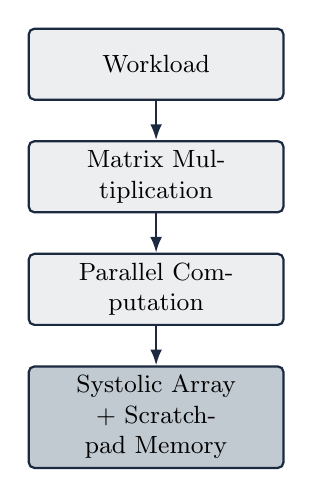
\begin{tikzpicture}[node distance=0.5cm]
        \node[block=3cm] (a) {Workload};
        \node[block=3cm, below=of a] (b) {Matrix Multiplication};
        \node[block=3cm, below=of b] (c) {Parallel Computation};
        \node[block=3cm, below=of c, fill=glight] (d) {Systolic Array \\ + Scratchpad Memory};
        \draw[darrow] (a)--(b); \draw[darrow] (b)--(c); \draw[darrow] (c)--(d);
      \end{tikzpicture}
    \end{column}
  \end{columns}
\end{frame}

% ============================================================
\begin{frame}{Why Systolic Arrays and Scratchpad Memory?}
  \begin{columns}[T]
    \begin{column}{0.52\textwidth}
      \begin{enumerate}
        \item \textbf{Parallelism} -- multiple PEs compute concurrently.
        \item \textbf{Data Reuse} -- data reused across computations instead of repeated external fetches.
        \item \textbf{Local Communication} -- PEs talk mainly to neighbors, reducing global data movement.
        \item \textbf{Predictable Dataflow} -- regular movement suits structured workloads (matmul, CNNs).
      \end{enumerate}
      \vspace{2mm}
      {\small \textit{Note: benefit depends on workload dimensions, dataflow mapping, memory bandwidth, and array size -- not automatic in every case.}}
    \end{column}
    \begin{column}{0.45\textwidth}
      \centering
      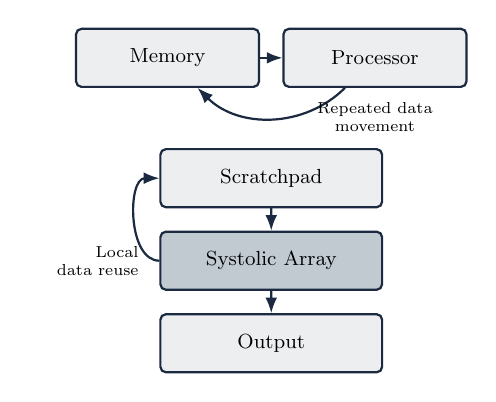
\begin{tikzpicture}[scale=0.82, every node/.style={transform shape}, node distance=0.35cm]
        \node[block=2.6cm] (m1) {Memory};
        \node[block=2.6cm, right=of m1] (p1) {Processor};
        \draw[darrow] (m1)--(p1);
        \draw[darrow] (p1) to[bend left=45] (m1);
        \node[below=0.1cm of p1, font=\scriptsize, text width=2.6cm, align=center] {Repeated data movement};
        \coordinate (mid) at ($(m1)!0.5!(p1)$);

        \node[block=3.2cm, below=1.4cm of mid] (s1) {Scratchpad};
        \node[block=3.2cm, below=of s1, fill=glight] (s2) {Systolic Array};
        \node[block=3.2cm, below=of s2] (s3) {Output};
        \draw[darrow] (s1)--(s2); \draw[darrow] (s2)--(s3);
        \draw[darrow] (s2) to[out=180,in=180] (s1);
        \node[left=0.2cm of s2, font=\scriptsize, text width=1.6cm, align=right] {Local data reuse};
      \end{tikzpicture}
    \end{column}
  \end{columns}
\end{frame}

% ============================================================
\begin{frame}{Literature Review}
  \footnotesize
  \renewcommand{\arraystretch}{1.15}
  \begin{tabular}{p{2.6cm}p{1.5cm}p{4.1cm}p{4.1cm}}
    \toprule
    \textbf{Paper} & \textbf{Year} & \textbf{Core Contributions} & \textbf{Limitations} \\
    \midrule
    Kung \& Leiserson -- \textit{Systolic Arrays for VLSI} &
    1978 &
    Introduced the systolic-array concept: a regular PE network for matrix computations &
    Purely conceptual/theoretical; no scratchpad, programmability, or CNN-specific dataflow \\[4pt]

    Jouppi et al. -- \textit{In-Datacenter Performance Analysis of a TPU} &
    2017 &
    Large-scale, fixed-function systolic array for datacenter ML inference &
    Fixed (weight-stationary) dataflow; limited flexibility across workload shapes; not open-sourced \\[4pt]

    Chen et al. -- \textit{Eyeriss} &
    2017 &
    Row-stationary dataflow for energy-efficient CNN data reuse &
    Array and dataflow tuned specifically to CNNs; less suited to irregular workloads \\[4pt]

    Kwon et al. -- \textit{MAERI} &
    2018 &
    Reconfigurable interconnect enabling flexible dataflow mapping &
    Added interconnect/control complexity and routing overhead vs.\ a simple mesh \\[4pt]

     Abdelmaksoud et al. -- \textit{DiP} &
    2024 &
    Scalable, energy-efficient systolic array design improving throughput for the weight-stationary dataflow &
    Optimized specifically for weight-stationary; not evaluated across other dataflow classes \\[4pt]
    \bottomrule
  \end{tabular}
\end{frame}

% ============================================================
\begin{frame}{Limitations and Design Challenges}
  \begin{columns}[T]
    \begin{column}{0.55\textwidth}
      \begin{itemize}
        \item \textbf{PE Utilization} -- large arrays under-utilized for small/irregular workloads.
        \item \textbf{Memory Bandwidth} -- compute can be limited by data supply rate.
        \item \textbf{Data Movement} -- moving activations, weights, partial sums is a major challenge.
        \item \textbf{Fixed Dataflow} -- architectures tuned for one dataflow may suit others poorly.
        \item \textbf{Scalability} -- larger arrays raise memory, routing, and control complexity.
        \item \textbf{Scratchpad Organization} -- size, banking, and access patterns affect reuse.
      \end{itemize}
    \end{column}
    \begin{column}{0.4\textwidth}
      \centering
      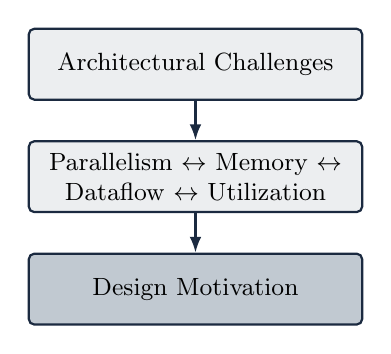
\begin{tikzpicture}[node distance=0.5cm]
        \node[block=4cm] (t) {Architectural Challenges};
        \node[block=4cm, below=of t] (m) {Parallelism $\leftrightarrow$ Memory $\leftrightarrow$ Dataflow $\leftrightarrow$ Utilization};
        \node[block=4cm, below=of m, fill=glight] (d) {Design Motivation};
        \draw[darrow] (t)--(m); \draw[darrow] (m)--(d);
      \end{tikzpicture}
    \end{column}
  \end{columns}
\end{frame}

% ============================================================
\begin{frame}{System-Level Architecture}
  \centering
  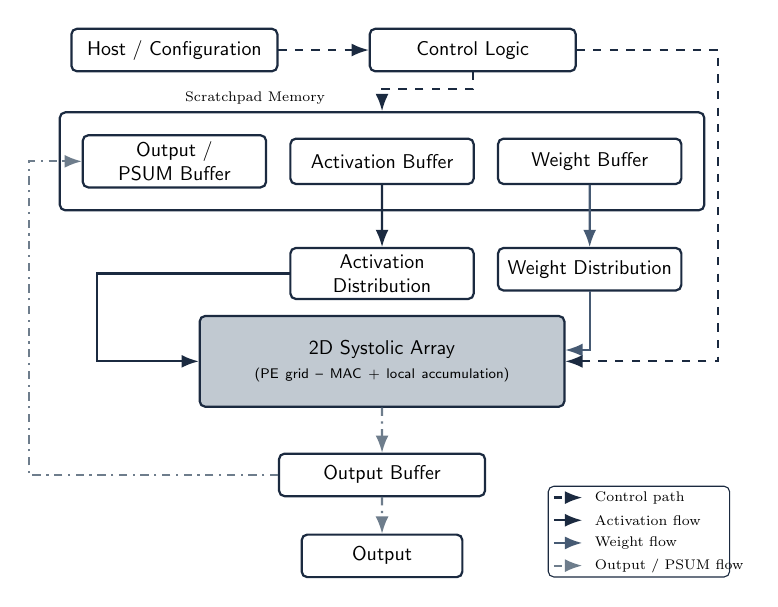
\begin{tikzpicture}[
      font=\sffamily,
      scale=0.72, every node/.style={transform shape},
      node distance=0.65cm and 0.5cm
    ]
    
    % Top row: Host and Control
    \node[sysblock=3.4cm] (host) {Host / Configuration};
    \node[sysblock=3.4cm, right=1.6cm of host] (ctrl) {Control Logic};

    % Scratchpad with sub-buffers
    \node[sysblock=3cm, minimum height=0.8cm, below=1.1cm of host] (outbuf) {Output / PSUM Buffer};
    \node[sysblock=3cm, minimum height=0.8cm, right=0.4cm of outbuf] (actbuf) {Activation Buffer};
    \node[sysblock=3cm, minimum height=0.8cm, right=0.4cm of actbuf] (wtbuf) {Weight Buffer};
    \node[draw=gdark, thick, rounded corners=2pt, fit=(actbuf)(wtbuf)(outbuf), inner sep=8pt, label={[font=\scriptsize]above left:Scratchpad Memory}] (spm) {};

    % Data distribution
    \node[sysblock=3cm, below=1.1cm of actbuf] (distA) {Activation Distribution};
    \node[sysblock=3cm, below=1.1cm of wtbuf] (distW) {Weight Distribution};

    % Systolic array
    \node[sysblock=6.2cm, minimum height=1.6cm, below=2.3cm of actbuf, fill=glight] (arr) {2D Systolic Array \\ \scriptsize (PE grid -- MAC + local accumulation)};

    % Output
    \node[sysblock=3.4cm, below=0.8cm of arr] (ob) {Output Buffer};
    \node[sysblock=2.6cm, below=of ob] (out) {Output};

    % Control path (dashed)
    \draw[ctrlarrow] (host) -- (ctrl);
    \draw[ctrlarrow] (ctrl.south) -- ++(0,-0.3) -| (spm.north);
    \draw[ctrlarrow] (ctrl.east) -- ++(2.5,0) |- (arr.east);

    % Activation flow (dark, solid)
    \draw[actarrow] (actbuf.south) -- (distA);
    \draw[actarrow] (distA.west) -- ++(-3.4,0) |- (arr.west);

    % Weight flow (grey, solid)
    \draw[wtarrow] (wtbuf) -- (distW);
    \draw[wtarrow] (distW.south) |- ([yshift=2mm]arr.east);

    % Output / partial-sum flow (dash-dot)
    \draw[outarrow] (arr) -- (ob);
    \draw[outarrow] (ob) -- (out);
    \draw[outarrow] (ob.west) -- ++(-4.4,0) |- (outbuf.west);

    % Legend
    \begin{scope}[shift={($(ob.east)+(1.2, -0.6)$)}]
      \draw[draw=gdark, rounded corners=2pt, fill=white] (-0.1, 0.4) rectangle (3.1, -1.2);
      \draw[ctrlarrow] (0.0,  0.2) -- (0.5,  0.2); \node[anchor=west, font=\scriptsize] at (0.6,  0.2) {Control path};
      \draw[actarrow]  (0.0, -0.2) -- (0.5, -0.2); \node[anchor=west, font=\scriptsize] at (0.6, -0.2) {Activation flow};
      \draw[wtarrow]   (0.0, -0.6) -- (0.5, -0.6); \node[anchor=west, font=\scriptsize] at (0.6, -0.6) {Weight flow};
      \draw[outarrow]  (0.0, -1.0) -- (0.5, -1.0); \node[anchor=west, font=\scriptsize] at (0.6, -1.0) {Output / PSUM flow};
    \end{scope}
  \end{tikzpicture}
\end{frame}

% ============================================================
\begin{frame}{Processing Element and Array}
  \begin{columns}[T]
    \begin{column}{0.4\textwidth}
      \centering
      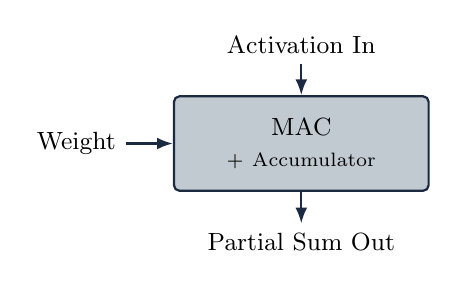
\begin{tikzpicture}[node distance=0.4cm]
        \node[font=\small] (ain) {Activation In};
        \node[block=3cm, below=of ain, fill=glight, minimum height=1.2cm] (mac) {MAC \\ \scriptsize + Accumulator};
        \node[font=\small, below=of mac] (pout) {Partial Sum Out};
        \node[font=\small, left=0.6cm of mac] (win) {Weight};
        \draw[darrow] (ain)--(mac);
        \draw[darrow] (mac)--(pout);
        \draw[darrow] (win)--(mac);
      \end{tikzpicture}
    \end{column}
    \begin{column}{0.55\textwidth}
      \centering
      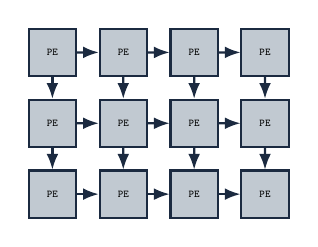
\begin{tikzpicture}[scale=0.75, every node/.style={transform shape}]
        \foreach \x in {0,1,2,3} {
          \foreach \y in {0,1,2} {
            \node[pe] (pe-\x-\y) at (\x*1.2, \y*1.2) {PE};
          }
        }
        \foreach \x in {0,1,2,3} {
          \foreach \y in {0,1} {
            \pgfmathtruncatemacro{\yn}{\y+1}
            \draw[darrow] (pe-\x-\yn) -- (pe-\x-\y);
          }
        }
        \foreach \y in {0,1,2} {
          \foreach \x in {0,1,2} {
            \pgfmathtruncatemacro{\xn}{\x+1}
            \draw[darrow] (pe-\x-\y) -- (pe-\xn-\y);
          }
        }
      \end{tikzpicture}
      \vspace{1mm} \\
      {\scriptsize Activations and weights propagate between neighboring PEs; partial sums accumulate locally.}
    \end{column}
  \end{columns}
  \vspace{1cm} 
  {\small Each PE performs local computation; regular structure enables spatial parallelism. \textit{Exact dataflow direction reflects the project's RTL.}}
\end{frame}

% ============================================================
\begin{frame}{Pipelined MAC Datapath (Computer Architecture View)}
  \centering
  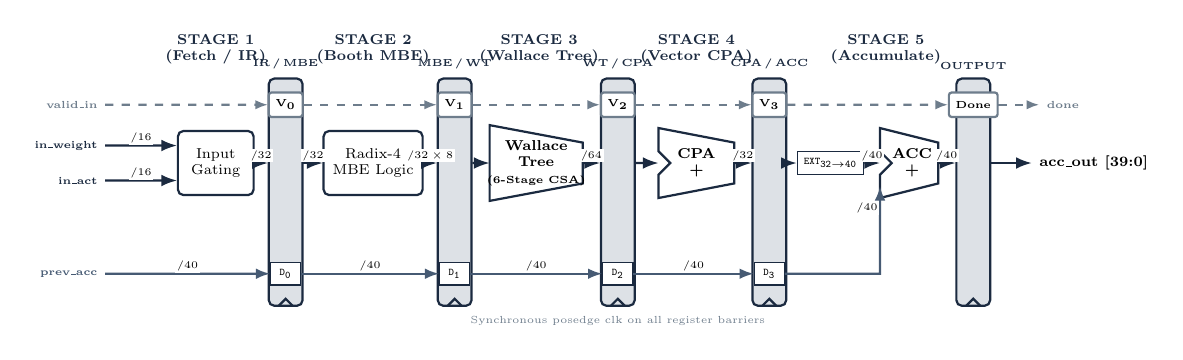
\begin{tikzpicture}[
      font=\sffamily,
      scale=0.74, every node/.style={transform shape},
      % Styles
      pipebar/.style={draw=gdark, thick, fill=glight!55, rounded corners=2pt, minimum width=0.58cm},
      pipetitle/.style={font=\tiny\bfseries, text=gdark, anchor=south},
      ctrlbox/.style={draw=gaccent, thick, fill=white, font=\tiny\bfseries, minimum size=0.42cm, rounded corners=1pt},
      regfield/.style={draw=gdark, thin, fill=white, font=\tiny\ttfamily, minimum width=0.52cm, minimum height=0.38cm},
      dpath/.style={-{Latex[length=2mm]}, thick, draw=gdark},
      cpath/.style={-{Latex[length=1.6mm]}, thick, dashed, draw=gaccent},
      accpath/.style={-{Latex[length=1.8mm]}, thick, draw=gmed},
      bus/.style={font=\tiny, fill=white, inner sep=0.8pt},
      stagelbl/.style={font=\scriptsize\bfseries, text=gdark, align=center}
    ]

    % Stage Column Headers (Top)
    \node[stagelbl] at (0.8,  2.85) {STAGE 1\\(Fetch / IR)};
    \node[stagelbl] at (3.5,  2.85) {STAGE 2\\(Booth MBE)};
    \node[stagelbl] at (6.35, 2.85) {STAGE 3\\(Wallace Tree)};
    \node[stagelbl] at (9.05, 2.85) {STAGE 4\\(Vector CPA)};
    \node[stagelbl] at (12.3, 2.85) {STAGE 5\\(Accumulate)};

    % Vertical Pipeline Register Slabs (Hennessy & Patterson style)
    \node[pipebar, minimum height=3.9cm] (preg1) at (2.0, 0.4) {};
    \node[pipetitle] at (2.0, 2.38) {IR\,/\,MBE};

    \node[pipebar, minimum height=3.9cm] (preg2) at (4.9, 0.4) {};
    \node[pipetitle] at (4.9, 2.38) {MBE\,/\,WT};

    \node[pipebar, minimum height=3.9cm] (preg3) at (7.7, 0.4) {};
    \node[pipetitle] at (7.7, 2.38) {WT\,/\,CPA};

    \node[pipebar, minimum height=3.9cm] (preg4) at (10.3, 0.4) {};
    \node[pipetitle] at (10.3, 2.38) {CPA\,/\,ACC};

    \node[pipebar, minimum height=3.9cm] (preg5) at (13.8, 0.4) {};
    \node[pipetitle] at (13.8, 2.38) {OUTPUT};

    % TOP TIER: Control Pipeline (valid_in -> done)
    \node[ctrlbox] (v0) at (2.0, 1.9) {V\textsubscript{0}};
    \node[ctrlbox] (v1) at (4.9, 1.9) {V\textsubscript{1}};
    \node[ctrlbox] (v2) at (7.7, 1.9) {V\textsubscript{2}};
    \node[ctrlbox] (v3) at (10.3, 1.9) {V\textsubscript{3}};
    \node[ctrlbox] (vd) at (13.8, 1.9) {Done};

    \draw[cpath] (-1.1, 1.9) node[left, font=\tiny\bfseries, text=gaccent]{valid\_in} -- (v0);
    \draw[cpath] (v0) -- (v1);
    \draw[cpath] (v1) -- (v2);
    \draw[cpath] (v2) -- (v3);
    \draw[cpath] (v3) -- (vd);
    \draw[cpath] (vd.east) -- ++(0.7,0) node[right, font=\tiny\bfseries, text=gaccent]{done};

    % MIDDLE TIER: Arithmetic Execution Datapath
    % Stage 1: Input Latch
    \node[draw=gdark, thick, fill=white, rounded corners=2pt, font=\scriptsize, minimum width=1.3cm, minimum height=1.1cm, align=center] (ir) at (0.8, 0.9) {Input\\Gating};
    \draw[dpath] (-1.1, 1.2) node[left, font=\tiny\bfseries, text=gdark]{in\_weight} -- node[above, bus]{/16} ([yshift=3mm]ir.west);
    \draw[dpath] (-1.1, 0.6) node[left, font=\tiny\bfseries, text=gdark]{in\_act}    -- node[above, bus]{/16} ([yshift=-3mm]ir.west);
    \draw[dpath] (ir) -- node[above, bus]{/32} (preg1.west |- ir);

    % Stage 2: Radix-4 Booth MBE
    \node[draw=gdark, thick, fill=white, rounded corners=2pt, font=\scriptsize, minimum width=1.7cm, minimum height=1.1cm, align=center] (mbe) at (3.5, 0.9) {Radix-4\\MBE Logic};
    \draw[dpath] (preg1.east |- ir) -- node[above, bus]{/32} (mbe.west);
    \draw[dpath] (mbe.east) -- node[above, bus]{/$32\times 8$} (preg2.west |- mbe);

    % Stage 3: Wallace Tree (Funnel Compressor Shape: 8:2)
    \draw[thick, fill=white, draw=gdark] 
      (5.5, 1.55) -- (7.1, 1.25) -- (7.1, 0.55) -- (5.5, 0.25) -- cycle;
    \node at (6.3, 0.9) [align=center, font=\scriptsize\bfseries] {Wallace\\Tree\\\tiny (6-Stage CSA)};
    \draw[dpath] (preg2.east |- mbe) -- (5.5, 0.9);
    \draw[dpath] (7.1, 0.9) -- node[above, bus]{/64} (preg3.west |- mbe);

    % Stage 4: Carry-Propagate Adder (ALU Chevron Shape)
    \draw[thick, fill=white, draw=gdark]
      (8.4, 1.5) -- (9.7, 1.25) -- (9.7, 0.55) -- (8.4, 0.3) -- (8.4, 0.7) -- (8.6, 0.9) -- (8.4, 1.1) -- cycle;
    \node at (9.05, 0.9) [align=center, font=\scriptsize\bfseries] {CPA\\+};
    \draw[dpath] (preg3.east |- mbe) -- (8.4, 0.9);
    \draw[dpath] (9.7, 0.9) -- node[above, bus]{/32} (preg4.west |- mbe);

    % Stage 5: Sign Extension & 40-bit Accumulator ALU
    \node[draw=gdark, thin, fill=white, font=\tiny\ttfamily] (ext) at (11.35, 0.9) {EXT\textsubscript{32$\to$40}};
    \draw[dpath] (preg4.east |- mbe) -- (ext.west);

    \draw[thick, fill=white, draw=gdark]
      (12.2, 1.5) -- (13.2, 1.25) -- (13.2, 0.55) -- (12.2, 0.3) -- (12.2, 0.7) -- (12.4, 0.9) -- (12.2, 1.1) -- cycle;
    \node at (12.75, 0.9) [align=center, font=\scriptsize\bfseries] {ACC\\+};
    \draw[dpath] (ext.east) -- node[above, bus]{/40} (12.2, 0.9);
    \draw[dpath] (13.2, 0.9) -- node[above, bus]{/40} (preg5.west |- mbe);
    \draw[dpath] (preg5.east |- mbe) -- ++(0.7,0) node[right, font=\scriptsize\bfseries]{acc\_out [39:0]};

    % BOTTOM TIER: Accumulator Delay Pipeline (prev_acc_buf[0..3])
    \node[regfield] (d0) at (2.0, -1.0) {D\textsubscript{0}};
    \node[regfield] (d1) at (4.9, -1.0) {D\textsubscript{1}};
    \node[regfield] (d2) at (7.7, -1.0) {D\textsubscript{2}};
    \node[regfield] (d3) at (10.3, -1.0) {D\textsubscript{3}};

    \draw[accpath] (-1.1, -1.0) node[left, font=\tiny\bfseries, text=gmed]{prev\_acc} -- node[above, bus]{/40} (d0);
    \draw[accpath] (d0) -- node[above, bus]{/40} (d1);
    \draw[accpath] (d1) -- node[above, bus]{/40} (d2);
    \draw[accpath] (d2) -- node[above, bus]{/40} (d3);

    % Route D3 up into the Stage 5 Accumulator input port
    \draw[accpath] (d3.east) -- (12.2, -1.0) -- node[near end, left, bus]{/40} (12.2, 0.5);

    % Clock ticks on pipeline register bases
    \foreach \x in {2.0, 4.9, 7.7, 10.3, 13.8} {
      \draw[thick, draw=gdark] (\x-0.12, -1.55) -- (\x, -1.43) -- (\x+0.12, -1.55);
    }
    \node[anchor=north, font=\tiny, text=gaccent] at (7.7, -1.6) {Synchronous posedge clk on all register barriers};

  \end{tikzpicture}

  \vspace{1mm}
  \begin{columns}[T]
    \begin{column}{0.48\textwidth}
      \scriptsize
      \textbf{Pipelined Microarchitectural Breakdown:}
      \begin{itemize}\scriptsize
        \item \textbf{Cycle 1 (Fetch/IR):} Dual 16-bit operand register latch.
        \item \textbf{Cycle 2 (Booth MBE):} Radix-4 recoding $\to$ 8 partial products.
        \item \textbf{Cycle 3 (Wallace Tree):} 6-stage CSA reduces $8 \to 2$ vectors ($O(\log N)$).
      \end{itemize}
    \end{column}
    \begin{column}{0.48\textwidth}
      \scriptsize
      \textbf{Timing \& Datapath Balancing:}
      \begin{itemize}\scriptsize
        \item \textbf{Cycle 4 (Merge CPA):} Final 32-bit Carry-Propagate Adder.
        \item \textbf{Cycle 5 (Accumulate):} 40-bit saturation-safe accumulation.
        \item \textbf{Hazard Prevention:} 4-stage FIFO ($D_0 \to D_3$) aligns \texttt{prev\_acc}.
      \end{itemize}
    \end{column}
  \end{columns}
\end{frame}

% ============================================================
\begin{frame}{Weight-Stationary (WS) Dataflow -- Detailed}
  \begin{columns}[T]
    % Left: array-level diagram
    \begin{column}{0.55\textwidth}
      \centering
      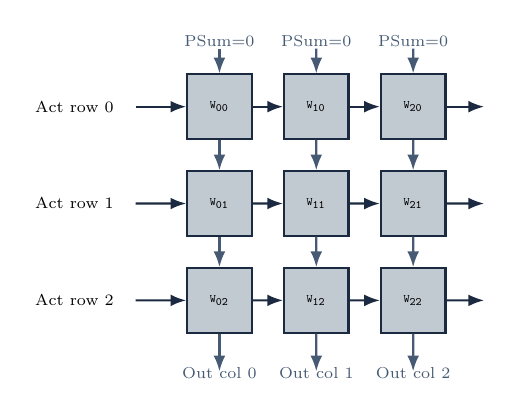
\begin{tikzpicture}[scale=0.82, every node/.style={transform shape}]
        \foreach \x in {0,1,2} {
          \foreach \y in {0,1,2} {
            \node[pe, minimum size=1cm] (pe-\x-\y) at (\x*1.5, -\y*1.5) {W\textsubscript{\x\y}};
          }
        }

        \foreach \y in {0,1,2} {
          \draw[darrow] (-1.3,-\y*1.5) -- (pe-0-\y)
            node[midway, above, font=\scriptsize] {};
          \draw[darrow] (pe-0-\y) -- (pe-1-\y);
          \draw[darrow] (pe-1-\y) -- (pe-2-\y);
          \draw[darrow] (pe-2-\y) -- ++(1.1,0);
        }
        \node[left=1cm of pe-0-0, font=\scriptsize] {Act row 0};
        \node[left=1cm of pe-0-1, font=\scriptsize] {Act row 1};
        \node[left=1cm of pe-0-2, font=\scriptsize] {Act row 2};

        \foreach \x in {0,1,2} {
          \draw[arrow] (\x*1.5,0.9) -- (pe-\x-0)
            node[midway, left, font=\scriptsize]{};
          \draw[arrow] (pe-\x-0) -- (pe-\x-1);
          \draw[arrow] (pe-\x-1) -- (pe-\x-2);
          \draw[arrow] (pe-\x-2) -- ++(0,-1.1);
        }
        \node[above=0.3cm of pe-0-0, font=\scriptsize, text=gmed] {PSum=0};
        \node[above=0.3cm of pe-1-0, font=\scriptsize, text=gmed] {PSum=0};
        \node[above=0.3cm of pe-2-0, font=\scriptsize, text=gmed] {PSum=0};
        \node[below=0.4cm of pe-0-2, font=\scriptsize, text=gmed] {Out col 0};
        \node[below=0.4cm of pe-1-2, font=\scriptsize, text=gmed] {Out col 1};
        \node[below=0.4cm of pe-2-2, font=\scriptsize, text=gmed] {Out col 2};
      \end{tikzpicture}
    \end{column}

    % Right: explanation
    \begin{column}{0.42\textwidth}
      \small
      \textbf{Stationary operand:} Weight \\
      Each PE loads one weight value once, and holds it for the entire computation -- it never moves again until the next weight tile is loaded.

      \vspace{2mm}
      \textbf{Streaming operands:}
      \begin{itemize}\small
        \item \textbf{Activations} -- move left $\to$ right, one row feeding each PE row
        \item \textbf{Partial sums} -- move top $\to$ bottom, accumulating down each PE column
      \end{itemize}
    \end{column}
  \end{columns}
  \vspace{2mm}
  \textbf{Why it helps:} weight reuse is maximized -- each weight is read from the scratchpad once and reused for every activation that streams past it, cutting weight-memory traffic.

  \vspace{3mm}
  \centering
  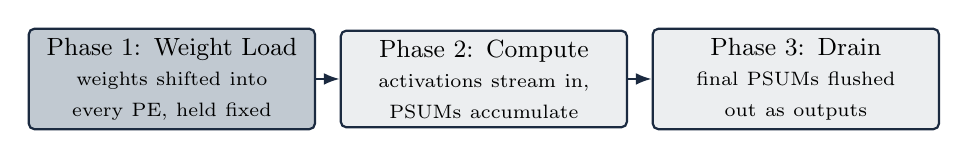
\begin{tikzpicture}[node distance=0.3cm]
    \node[block=3.4cm, fill=glight] (p1) {Phase 1: Weight Load \\ \scriptsize weights shifted into every PE, held fixed};
    \node[block=3.4cm, right=of p1] (p2) {Phase 2: Compute \\ \scriptsize activations stream in, PSUMs accumulate};
    \node[block=3.4cm, right=of p2] (p3) {Phase 3: Drain \\ \scriptsize final PSUMs flushed out as outputs};
    \draw[darrow] (p1)--(p2);
    \draw[darrow] (p2)--(p3);
  \end{tikzpicture}
\end{frame}

% ============================================================
\begin{frame}{Control and Execution Flow}
  \begin{columns}[T]
    \begin{column}{0.45\textwidth}
      \centering
      \scriptsize\textit{Conceptual execution flow}
      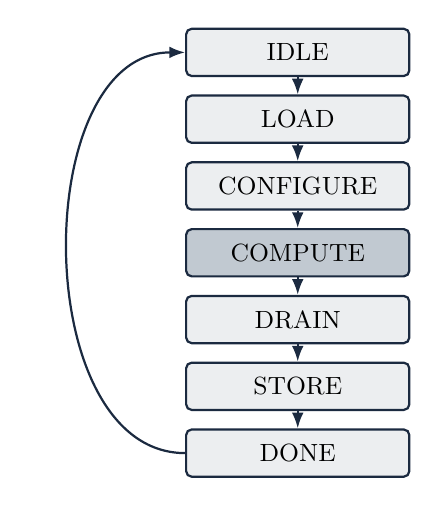
\begin{tikzpicture}[node distance=0.22cm]
        \node[block=2.6cm, minimum height=0.6cm] (idle) {IDLE};
        \node[block=2.6cm, minimum height=0.6cm, below=of idle] (load) {LOAD};
        \node[block=2.6cm, minimum height=0.6cm, below=of load] (cfg) {CONFIGURE};
        \node[block=2.6cm, minimum height=0.6cm, below=of cfg, fill=glight] (comp) {COMPUTE};
        \node[block=2.6cm, minimum height=0.6cm, below=of comp] (drain) {DRAIN};
        \node[block=2.6cm, minimum height=0.6cm, below=of drain] (store) {STORE};
        \node[block=2.6cm, minimum height=0.6cm, below=of store] (done) {DONE};
        \draw[darrow] (idle)--(load); \draw[darrow] (load)--(cfg);
        \draw[darrow] (cfg)--(comp); \draw[darrow] (comp)--(drain);
        \draw[darrow] (drain)--(store); \draw[darrow] (store)--(done);
        \draw[darrow] (done) to[out=180,in=180] (idle);
      \end{tikzpicture}
    \end{column}
    \begin{column}{0.5\textwidth}
      \centering
      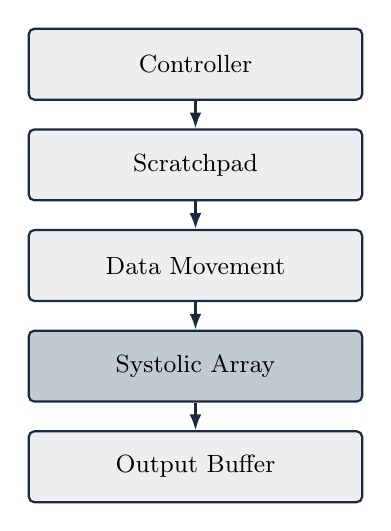
\begin{tikzpicture}[node distance=0.35cm]
        \node[block=4cm] (c) {Controller};
        \node[block=4cm, below=of c] (s) {Scratchpad};
        \node[block=4cm, below=of s] (d) {Data Movement};
        \node[block=4cm, below=of d, fill=glight] (a) {Systolic Array};
        \node[block=4cm, below=of a] (o) {Output Buffer};
        \draw[darrow] (c)--(s); \draw[darrow] (s)--(d);
        \draw[darrow] (d)--(a); \draw[darrow] (a)--(o);
      \end{tikzpicture}
      \vspace{2mm}\\
      {\scriptsize Configuration $\to$ data load $\to$ compute start $\to$ pipeline fill $\to$ compute $\to$ pipeline drain $\to$ store $\to$ completion signal.}
    \end{column}
  \end{columns}
  \vspace{1mm}
  {\scriptsize FSM states shown are conceptual unless they match the implemented RTL exactly.}
\end{frame}

% ============================================================
\begin{frame}{RTL Implementation and Verification}
  \begin{columns}[T]
    \begin{column}{0.42\textwidth}
      \centering
      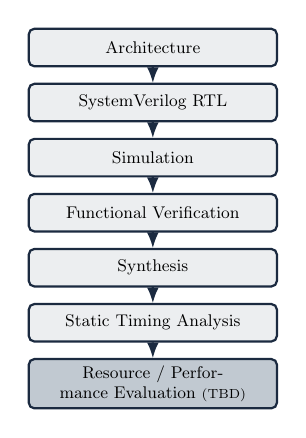
\begin{tikzpicture}[node distance=0.14cm, scale=0.68, every node/.style={transform shape}]
        \node[block=4.4cm, minimum height=0.7cm] (a) {Architecture};
        \node[block=4.4cm, minimum height=0.7cm, below=0.3cm of a] (b) {SystemVerilog RTL};
        \node[block=4.4cm, minimum height=0.7cm, below=0.3cm of b] (c) {Simulation};
        \node[block=4.4cm, minimum height=0.7cm, below=0.3cm of c] (d) {Functional Verification};
        \node[block=4.4cm, minimum height=0.7cm, below=0.3cm of d] (e) {Synthesis};
        \node[block=4.4cm, minimum height=0.7cm, below=0.3cm of e] (f) {Static Timing Analysis};
        \node[block=4.4cm, minimum height=0.9cm, below=0.3cm of f, fill=glight] (g) {Resource / Performance Evaluation \scriptsize (TBD)};
        \foreach \s/\t in {a/b,b/c,c/d,d/e,e/f,f/g} { \draw[darrow] (\s)--(\t); }
      \end{tikzpicture}
    \end{column}
    \begin{column}{0.54\textwidth}
      \small \textbf{Tools} (where used): \\
      Verilator / Icarus Verilog, GTKWave, Yosys, OpenSTA
      \vspace{3mm}

      \small \textbf{Verification scope:} \\
      PE-level, array-level, scratchpad, end-to-end, corner cases, pipeline/data alignment
      \vspace{3mm}

    \end{column}
  \end{columns}
\end{frame}

% ============================================================
\begin{frame}{Contribution and Future Work}
  \begin{columns}[T]
    \begin{column}{0.48\textwidth}
      \textbf{\small Project Contribution}
      \begin{itemize}\small
        \item 2D systolic-array architecture
        \item Modular Processing Elements
        \item Scratchpad-based local storage
        \item Programmable control / data movement
        \item Synthesizable RTL architecture
        \item Verification and evaluation methodology
      \end{itemize}
    \end{column}
    \begin{column}{0.48\textwidth}
      \textbf{\small Future Work}
      \begin{itemize}\small
        \item Double buffering
        \item DMA-based data movement
        \item Improved scratchpad banking
        \item AXI / APB interface
        \item Multiple numerical precisions
        \item Larger / scalable arrays
        \item FPGA optimization, ASIC implementation
      \end{itemize}
    \end{column}
  \end{columns}
  \vspace{3mm}
  \begin{block}{Conclusion}
    \small A programmable spatial architecture combining \textbf{parallel computation + local data reuse + structured data movement}.
  \end{block}
  \vspace{4mm}
  \centering \Large \textbf{Thank You} \\ \normalsize 
\end{frame}

\end{document}
